\documentclass[a4paper,10pt,twoside]{article}
\usepackage{a4wide}
\usepackage[utf8]{inputenc}
\usepackage[spanish,es-noshorthands,es-ucroman]{babel} % Opciones luego de spanish por problema de compatibilidad con csvsimple
\usepackage{setspace}        % Para setear el espacio entre lineas del título en la carátula
\usepackage{fancyhdr}
\usepackage{lastpage}
\usepackage{amsmath}
\usepackage{amsfonts}
\usepackage{verbatim}
\usepackage{graphicx}
\usepackage{blindtext}
\usepackage{floatrow}
\usepackage{csvsimple}
\usepackage{xstring}
\usepackage{xcolor}
\usepackage{listings}
\usepackage{tocbibind}


% Evita que el documento se estire verticalmente para ocupar
% el espacio vacío en cada página.
\raggedbottom


%%%%%%%%%% Configuración de Listings - Inicio %%%%%%%%%%
\definecolor{mygray}{rgb}{0.5,0.5,0.5}
\lstset{extendedchars=\true}
\lstdefinestyle{customc}{
	belowcaptionskip=1\baselineskip,
	breaklines=true,
	language=C++,
	showstringspaces=false,
	basicstyle=\footnotesize\ttfamily,
	keywordstyle=\bfseries\color{green!40!black},
	commentstyle=\itshape\color{purple!40!black},
	identifierstyle=\color{blue},
	stringstyle=\color{orange},
	numbers=left,
	numberstyle=\color{mygray}
}
\lstset{escapechar=@,style=customc}
%%%%%%%%%% Configuración de Listings - Fin %%%%%%%%%%


%%%%%%%%%% Configuración de Fancyhdr - Inicio %%%%%%%%%%
\pagestyle{fancy}
\thispagestyle{fancy}
\lhead{Estimación de Parámetros de la Distribución $\Gamma$ Generalizada}
\rhead{Capra, Lovisolo, Petaccio}
\renewcommand{\footrulewidth}{0.4pt}
\cfoot{\thepage /\pageref{LastPage}}

\fancypagestyle{caratula} {
   \fancyhf{}
   \cfoot{\thepage /\pageref{LastPage}}
   \renewcommand{\headrulewidth}{0pt}
   \renewcommand{\footrulewidth}{0pt}
}
%%%%%%%%%% Configuración de Fancyhdr - Fin %%%%%%%%%%


%%%%%%%%%% Macros para incluir gráficos - Inicio %%%%%%%%%%
% Inserta un gráfico centrado.
% Uso: \grafico{ruta al grafico .tex}{etiqueta}
\newcommand{\grafico}[2]{
	\begin{figure}[H]
		\caption{#2}
		\centering
		\input{#1}
	\end{figure}
}

% Inserta dos gráficos en fila.
% Uso: \graficodoble{ruta al grafico 1.tex}{etiqueta 1}{ruta al grafico 2.tex}{etiqueta 2}
\newcommand{\graficodoble}[4]{
	\begin{figure}[H]
		\begin{floatrow}
			\floatbox{figure}[.4\textwidth][\FBheight][t]
			{\caption{#2}}
			{\input{#1}}
			\hspace*{1cm}
			\floatbox{figure}[.4\textwidth][\FBheight][t]
			{\caption{#4}}
			{\input{#3}}
		\end{floatrow}
	\end{figure}	
}
%%%%%%%%%% Macros para incluir gráficos - Fin %%%%%%%%%%


%%%%%%%%%% Macro para incluir CSVs - Inicio %%%%%%%%%%
% Inserta una tabla con el contenido de un archivo CSV.
% Uso: \incluircsv{ruta al archivo.csv}{formato de columnas}{cabeza}{filas}
%
% Parámetros:
%   {formato de columnas} formato idéntico al usado en \begin{table}{...}.
%   {cabeza} el contenido de la primera fila de la tabla.
%   {filas} el contenido de cada fila individual.
%
% Ejemplo:
%
%   --- Archivo ejemplo.csv ---
%
%     Nombre,Apellido,Edad
%     Juan,Perez,30
%     María,Gomez,25
%     Pablo,Rodríguez,38
%
%   --- Código LaTeX ---
%
%     \incluircsv{ejemplo.csv}
%                {|r|l|}
%                {Sujeto & Edad}
%                {\Nombre \Apellido & \Edad}
%
%   --- Salida ---
%
%      +-----------------+------+
%      |          Sujeto | Edad |
%      +-----------------+------+
%      |      Juan Perez | 30   |
%      |     María Gomez | 25   |
%      | Pablo Rodríguez | 38   |
%      +-----------------+------+
\newcommand{\incluircsv}[4]{
	\begin{center}
		\csvreader[tabular=#2,
		           table head=\hline #3 \\\hline,
		           late after line=\\,
		           late after last line=\\\hline,
		           head to column names]
		          {#1}{}{#4}
	\end{center}              
}
%%%%%%%%%% Macro para incluir CSVs - Fin %%%%%%%%%%


%%%%%%%%%% Macros varios - Inicio %%%%%%%%%%
% Devuelve el nombre de una muestra dada la ruta al archivo correspondiente
% Uso: \nombremuestra{data/Xn.txt}
%
% Ejemplo: \nombremuesra{data/X1.txt}
% Salida: X1
\newcommand{\nombremuestra}[1]{%
	\let \nombre #1%
	\StrSubstitute{\nombre}{data/}{}[\nombre]%
	\StrSubstitute{\nombre}{data/tag}{}[\nombre]%
	\StrSubstitute{\nombre}{.txt}{}[\nombre]%
	\nombre%
}
%%%%%%%%%% Macros varios - Fin %%%%%%%%%%


\begin{document}


%%%%%%%%%%%%%%%%%%%%%%%%%%%%%%%%%%%%%%%%%%%%%%%%%%%%%%%%%%%%%%%%%%%%%%%%%%%%%%%
%% Carátula                                                                  %%
%%%%%%%%%%%%%%%%%%%%%%%%%%%%%%%%%%%%%%%%%%%%%%%%%%%%%%%%%%%%%%%%%%%%%%%%%%%%%%%


\thispagestyle{caratula}

\begin{center}

Departamento de Computación,\\
Facultad de Ciencias Exactas y Naturales,\\
Universidad de Buenos Aires

\begin{spacing}{2.5}
\begin{Huge}
Estimación de Parámetros de la\\
Distribución Gamma Generalizada
\end{Huge}
\end{spacing}

\vspace{1cm}

Trabajo Práctico 1, \\
Métodos Numéricos, \\
Primer Cuatrimestre de 2013

\vspace{1cm}


\includegraphics[width=5cm]{UBA.jpg} 

\vspace{1cm}

\begin{tabular}{|c|c|c|}
\hline
Apellido y Nombre & LU & E-mail\\
\hline
María Candela Capra Coarasa & 234/11 & canduh\_27@hotmail.com\\
Leandro Lovisolo            & 645/11 & leandro@leandro.me\\
Lautaro José Petaccio       & 443/11 & lausuper@gmail.com\\
\hline
\end{tabular}

\vspace{2cm}

\end{center}

\textbf{Resumen:} \\
Introducimos un método para estimar los parámetros de una D$\Gamma$G a partir de una muestra.
Utilizamos estimadores de máxima verosimilitud y cálculo de momentos para obtener un sistema
de ecuaciones no-lineal de los parámetros de la distribución, y aplicamos métodos de análisis
numérico (bisección y Newton) para aproximar una solución con un margen de error dado.

\textbf{Palabras claves:} D$\Gamma$G, estimadores, bisección, Newton.

\vspace{6cm}

\newpage


%%%%%%%%%%%%%%%%%%%%%%%%%%%%%%%%%%%%%%%%%%%%%%%%%%%%%%%%%%%%%%%%%%%%%%%%%%%%%%%
%% Índice                                                                    %%
%%%%%%%%%%%%%%%%%%%%%%%%%%%%%%%%%%%%%%%%%%%%%%%%%%%%%%%%%%%%%%%%%%%%%%%%%%%%%%%


\tableofcontents

\newpage


%%%%%%%%%%%%%%%%%%%%%%%%%%%%%%%%%%%%%%%%%%%%%%%%%%%%%%%%%%%%%%%%%%%%%%%%%%%%%%%
%% Introducción Teórica                                                      %%
%%%%%%%%%%%%%%%%%%%%%%%%%%%%%%%%%%%%%%%%%%%%%%%%%%%%%%%%%%%%%%%%%%%%%%%%%%%%%%%


\section{Introducción Teórica}

El objetivo de este trabajo es presentar un método para la aproximación de los
parámetros de una muestra que sigue la Distribución Gamma Generalizada
\footnote{Ver http://en.wikipedia.org/wiki/Generalized\_gamma\_distribution.}.

Esta distribución depende de tres parámetros $\sigma$, $\beta$ y $\lambda$ que siguen
las ecuaciones (1), (2) y (3) presentadas en el apéndice A.

Aplicando cálculo de momentos se obtiene la ecuación (4), una expresión para
el parámetro $\beta$ que sólo depende de la muestra. Hallando el valor de $\beta$
a partir de la ecuación (4) se pueden obtener fácilmente los valores de $\sigma$
y $\lambda$ reemplazando $\beta$ en las ecuaciones (1) y (2), respectivamente.

La problemática central en este trabajo yace en hallar un valor para el
parámetro $\beta$, que es imposible de despejar de la ecuación (4) por medio de
manipulación algebráica. Sin embargo, es posible aproximar el parámetro $\beta$
haciendo uso de métodos de aproximación numérica y a partir de éste hallar
aproximaciones de los parámetros restantes que ajustan a la muestra de forma
excelente.

Los métodos que exploramos son el \emph{método de bisección} \cite{burden}[p.~48]
y el \emph{método de Newton} \cite{burden}[p.~67], que introducimos a continuación.


\subsection{Método de bisección}
Teniendo una función $f(x)$ contínua en $[a,b]$ con $f(a).f(b) < 0$, es posible utilizar el Teorema del Valor Intermedio, el cual bajo estas hipótesis afirma la existencia de $c \in (a,b)$ tal que $f(c) = 0$. Conociendo la existencia de este c, se puede aplicar el método de bisección el cuál consiste en la división del intervalo [a,b] por su mitad (m) sucesivamente hasta conseguir un m para el cuál $f(m)$ sea 0 o lo suficientemente cercano al cero según el criterio de parada utilizado.
Para eligir el próximo intervalo sobre el cuál volver a realizar el procedimiento en cada iteración, se utiliza el siguiente criterio:

\begin{itemize}
    \item Si $f(m) = 0$ entonces ya tenemos el m que se buscaba.
    \item Si $f(a).f(m) < 0$ entonces se utiliza el intervalo $[a,m]$, si no, se utiliza $[m,b]$.
\end{itemize}

\subsection{Método de Newton}
Teniendo $f \in C^2[a,b]$ y $p_0 \in [a, b]$ siendo $p_0$ una aproximación al valor p buscado tal que $f'(p_0) \neq 0$, se toma la recta tangente a $f(x)$ en $p_0$ y al intersecarse con la recta $x = 0$ se obtiene el próximo $x_0$ con el cual volver a repetir la operación hasta encontrarse con alguna de las cotas establecidas para el algoritmo. \\
El algoritmo es el siguiente: 
\begin{equation*}
	p_n = p_{n-1} - \frac{f(p_{n-1})}{f'(p_{n-1})} , \qquad \text{para n} \geq 1
\end{equation*}
El algoritmo sólo puede asegurar convergencia si $f \in C^2[a,b] \land p \in (a,b)$ tal que $f(p) = 0 \land f'(p) \neq 0$ el método genera una sucesión convergente a p para cualquier $p_0$ inicial lo suficientemente cercano a p, es decir $p_0 \in [p-\delta,p+\delta]$.


%%%%%%%%%%%%%%%%%%%%%%%%%%%%%%%%%%%%%%%%%%%%%%%%%%%%%%%%%%%%%%%%%%%%%%%%%%%%%%%
%% Desarrollo                                                                %%
%%%%%%%%%%%%%%%%%%%%%%%%%%%%%%%%%%%%%%%%%%%%%%%%%%%%%%%%%%%%%%%%%%%%%%%%%%%%%%%


\section{Desarrollo}
Siendo nuestro objetivo estimar el parámetro $\beta$ y luego con este los demás, manipulamos la ecuación 4 provista por la cátedra para poder llegar a igualarla a 0. El sentido de esta manipulación es poder aprovechar los métodos de Newton y bisección elegidos, los cuales se utilizan para encontrar raíces, y utilizarlos para encontrar el $\beta$ que mejor aproxime la función al 0 el cual, por la manipulación de la ecuación que hicimos, sería el beta buscado.

Para obtener una primera noción de la ubicación del parámetro $\beta$ en la
recta real, aplicamos el método de bisección sobre todas las muestras en el
intervalo $[1, 100]$\footnote{Tomamos un intervalo arbitrariamente grande,
usando como heurística los parámetros de las muestras de referencia provistas
por la cátedra y la similitud del rango de valores de las mediciones de las
muestras de referencia y de las que se desean estimar.} con límites de 100
iteraciones y error absoluto $10^{-4}$, y precisión de 51 bits de mantisa.

En cada caso el método convergió a una solución luego de 20 iteraciones.
Una vez hallado $\beta$, despejamos los parámetros $\sigma$ y $\lambda$ y
dibujamos el histograma y función de densidad superpuestos. Se observa
excelente ajuste en todas las muestras.

Siguiendo un razonamiento similar, modificamos el experimento anterior,
esta vez aplicando el método de Newton, tomando como aproximación inicial
$\beta_0 = 10$ y manteniendo los mismos criterios de parada y precisión.

Observamos que el método converge a soluciones muy similares a las del
experimento inicial luego de 7 iteraciones en promedio, a excepción de la
muestra 3. Con esta última, el método converge a un valor muy pequeño de
$\beta$ que efectivamente anula la ecuación (4) pero no ajusta al histograma
de la muestra.

Para remendar esta situación, repetimos el experimento sobre la muestra 3
tomando como aproximación inicial la parte entera del valor de $\beta$ hallado
con el método de bisección. Observamos convergencia a una solución correcta
luego de 5 iteraciones.

Probando un poco más con la muestra 3, vimos que también convergía a una
solución correcta con $p_0 = 5$, realizamos la prueba con las demás muestras
y vimos que estas también lo hacían, por lo que fijamos un $p_0$ fijo para
nuestros experimentos en $p_0$ = 5.

Una vez hallados los parámetros de las distribuciones de cada muestra y un
conjunto de puntos de partida para los métodos que decidimos aplicar,
procedimos a explorar otras configuraciones. 

Evaluamos inicialmente cotas de error absoluto y relativo de 0.001, 0.01 y 0.1, y mantisas
de precisión de 51, 30 y 10 bits, de manera de tener una opción fina, regular y
grosera para cada valor.

Observamos que para mantisas de 10 bits, el método de Newton divergía con todas
las muestra, y el método de bisección producía valores erróneos. Además,
no observamos diferencias notables con mantisas de 30 bits, por lo cual reducimos
esa precisión hasta empezar a ver diferencias significativas. Por estos motivos
nos decidimos por valores de 51, 20 y 15 bits para los sucesivos experimentos.

Realizamos las pruebas y al encontrar valores muy similares con las mayores precisiones
de ambos métodos escogimos el método de Newton con cota de error absoluta 0.001 y 51 bits de mantisa
para plasmar en los gráficos cómo estos parámetros obtenidos aproximan la muestra.

Por último, comparamos las muestras usando todas las combinaciones de mantisas y criterios
de parada para elegir las que mejor ilustran las diferencias de estos ajustes, y
generamos gráficos comparativos dibujando las curvas de ajuste para distintos valores
sobre el mismo histograma.

Realizamos un estudio de función para corroborar que los $\beta$ obtenidos fueran los buscados.

\begin{figure}[H]
  \centering
  \caption{Estudio de la ecuación 4}
  % GNUPLOT: LaTeX picture with Postscript
\begingroup
  \makeatletter
  \providecommand\color[2][]{%
    \GenericError{(gnuplot) \space\space\space\@spaces}{%
      Package color not loaded in conjunction with
      terminal option `colourtext'%
    }{See the gnuplot documentation for explanation.%
    }{Either use 'blacktext' in gnuplot or load the package
      color.sty in LaTeX.}%
    \renewcommand\color[2][]{}%
  }%
  \providecommand\includegraphics[2][]{%
    \GenericError{(gnuplot) \space\space\space\@spaces}{%
      Package graphicx or graphics not loaded%
    }{See the gnuplot documentation for explanation.%
    }{The gnuplot epslatex terminal needs graphicx.sty or graphics.sty.}%
    \renewcommand\includegraphics[2][]{}%
  }%
  \providecommand\rotatebox[2]{#2}%
  \@ifundefined{ifGPcolor}{%
    \newif\ifGPcolor
    \GPcolorfalse
  }{}%
  \@ifundefined{ifGPblacktext}{%
    \newif\ifGPblacktext
    \GPblacktexttrue
  }{}%
  % define a \g@addto@macro without @ in the name:
  \let\gplgaddtomacro\g@addto@macro
  % define empty templates for all commands taking text:
  \gdef\gplbacktext{}%
  \gdef\gplfronttext{}%
  \makeatother
  \ifGPblacktext
    % no textcolor at all
    \def\colorrgb#1{}%
    \def\colorgray#1{}%
  \else
    % gray or color?
    \ifGPcolor
      \def\colorrgb#1{\color[rgb]{#1}}%
      \def\colorgray#1{\color[gray]{#1}}%
      \expandafter\def\csname LTw\endcsname{\color{white}}%
      \expandafter\def\csname LTb\endcsname{\color{black}}%
      \expandafter\def\csname LTa\endcsname{\color{black}}%
      \expandafter\def\csname LT0\endcsname{\color[rgb]{1,0,0}}%
      \expandafter\def\csname LT1\endcsname{\color[rgb]{0,1,0}}%
      \expandafter\def\csname LT2\endcsname{\color[rgb]{0,0,1}}%
      \expandafter\def\csname LT3\endcsname{\color[rgb]{1,0,1}}%
      \expandafter\def\csname LT4\endcsname{\color[rgb]{0,1,1}}%
      \expandafter\def\csname LT5\endcsname{\color[rgb]{1,1,0}}%
      \expandafter\def\csname LT6\endcsname{\color[rgb]{0,0,0}}%
      \expandafter\def\csname LT7\endcsname{\color[rgb]{1,0.3,0}}%
      \expandafter\def\csname LT8\endcsname{\color[rgb]{0.5,0.5,0.5}}%
    \else
      % gray
      \def\colorrgb#1{\color{black}}%
      \def\colorgray#1{\color[gray]{#1}}%
      \expandafter\def\csname LTw\endcsname{\color{white}}%
      \expandafter\def\csname LTb\endcsname{\color{black}}%
      \expandafter\def\csname LTa\endcsname{\color{black}}%
      \expandafter\def\csname LT0\endcsname{\color{black}}%
      \expandafter\def\csname LT1\endcsname{\color{black}}%
      \expandafter\def\csname LT2\endcsname{\color{black}}%
      \expandafter\def\csname LT3\endcsname{\color{black}}%
      \expandafter\def\csname LT4\endcsname{\color{black}}%
      \expandafter\def\csname LT5\endcsname{\color{black}}%
      \expandafter\def\csname LT6\endcsname{\color{black}}%
      \expandafter\def\csname LT7\endcsname{\color{black}}%
      \expandafter\def\csname LT8\endcsname{\color{black}}%
    \fi
  \fi
  \setlength{\unitlength}{0.0500bp}%
  \begin{picture}(7678.00,5280.00)%
    \gplgaddtomacro\gplbacktext{%
      \colorrgb{0.00,0.00,0.00}%
      \put(420,400){\makebox(0,0)[r]{\strut{}-1}}%
      \colorrgb{0.00,0.00,0.00}%
      \put(420,1063){\makebox(0,0)[r]{\strut{}0}}%
      \colorrgb{0.00,0.00,0.00}%
      \put(420,1725){\makebox(0,0)[r]{\strut{}1}}%
      \colorrgb{0.00,0.00,0.00}%
      \put(420,2388){\makebox(0,0)[r]{\strut{}2}}%
      \colorrgb{0.00,0.00,0.00}%
      \put(420,3051){\makebox(0,0)[r]{\strut{}3}}%
      \colorrgb{0.00,0.00,0.00}%
      \put(420,3714){\makebox(0,0)[r]{\strut{}4}}%
      \colorrgb{0.00,0.00,0.00}%
      \put(420,4376){\makebox(0,0)[r]{\strut{}5}}%
      \colorrgb{0.00,0.00,0.00}%
      \put(420,5039){\makebox(0,0)[r]{\strut{}6}}%
      \colorrgb{0.00,0.00,0.00}%
      \put(863,200){\makebox(0,0){\strut{}0}}%
      \colorrgb{0.00,0.00,0.00}%
      \put(2154,200){\makebox(0,0){\strut{}20}}%
      \colorrgb{0.00,0.00,0.00}%
      \put(3444,200){\makebox(0,0){\strut{}40}}%
      \colorrgb{0.00,0.00,0.00}%
      \put(4735,200){\makebox(0,0){\strut{}60}}%
      \colorrgb{0.00,0.00,0.00}%
      \put(6026,200){\makebox(0,0){\strut{}80}}%
      \colorrgb{0.00,0.00,0.00}%
      \put(7317,200){\makebox(0,0){\strut{}100}}%
    }%
    \gplgaddtomacro\gplfronttext{%
      \csname LTb\endcsname%
      \put(6414,1763){\makebox(0,0)[r]{\strut{}Muestra X1}}%
      \csname LTb\endcsname%
      \put(6414,1563){\makebox(0,0)[r]{\strut{}Muestra X2}}%
      \csname LTb\endcsname%
      \put(6414,1363){\makebox(0,0)[r]{\strut{}Muestra X3}}%
      \csname LTb\endcsname%
      \put(6414,1163){\makebox(0,0)[r]{\strut{}Muestra X4}}%
      \csname LTb\endcsname%
      \put(6414,963){\makebox(0,0)[r]{\strut{}Muestra X5}}%
      \csname LTb\endcsname%
      \put(6414,763){\makebox(0,0)[r]{\strut{}Muestra X6}}%
      \csname LTb\endcsname%
      \put(6414,563){\makebox(0,0)[r]{\strut{}Muestra X7}}%
    }%
    \gplbacktext
    \put(0,0){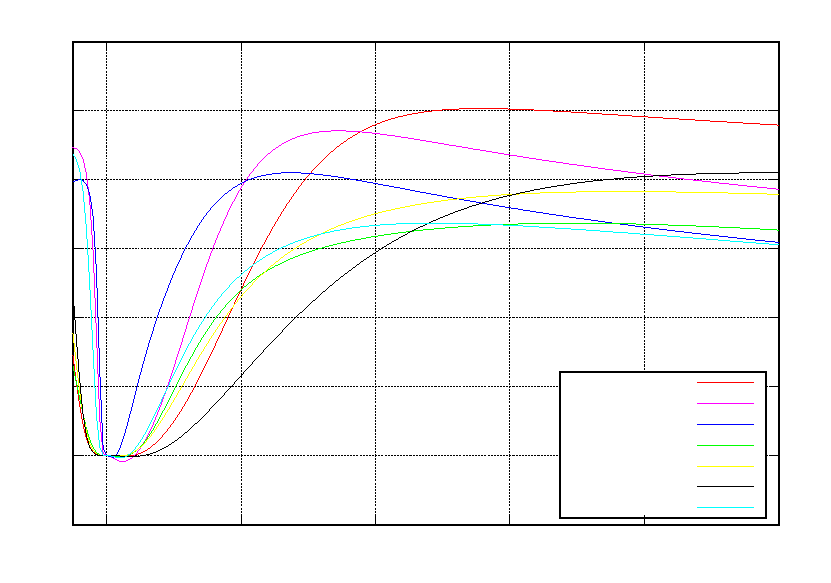
\includegraphics{grafico-ecuacion-4}}%
    \gplfronttext
  \end{picture}%
\endgroup

\end{figure}

Para poder apreciar correctamente el funcionamiento de los métodos, nos centramos en los ceros de la función.

\begin{figure}[H]
  \centering
  \caption{Ceros de la ecuación 4}
  % GNUPLOT: LaTeX picture with Postscript
\begingroup
  \makeatletter
  \providecommand\color[2][]{%
    \GenericError{(gnuplot) \space\space\space\@spaces}{%
      Package color not loaded in conjunction with
      terminal option `colourtext'%
    }{See the gnuplot documentation for explanation.%
    }{Either use 'blacktext' in gnuplot or load the package
      color.sty in LaTeX.}%
    \renewcommand\color[2][]{}%
  }%
  \providecommand\includegraphics[2][]{%
    \GenericError{(gnuplot) \space\space\space\@spaces}{%
      Package graphicx or graphics not loaded%
    }{See the gnuplot documentation for explanation.%
    }{The gnuplot epslatex terminal needs graphicx.sty or graphics.sty.}%
    \renewcommand\includegraphics[2][]{}%
  }%
  \providecommand\rotatebox[2]{#2}%
  \@ifundefined{ifGPcolor}{%
    \newif\ifGPcolor
    \GPcolorfalse
  }{}%
  \@ifundefined{ifGPblacktext}{%
    \newif\ifGPblacktext
    \GPblacktexttrue
  }{}%
  % define a \g@addto@macro without @ in the name:
  \let\gplgaddtomacro\g@addto@macro
  % define empty templates for all commands taking text:
  \gdef\gplbacktext{}%
  \gdef\gplfronttext{}%
  \makeatother
  \ifGPblacktext
    % no textcolor at all
    \def\colorrgb#1{}%
    \def\colorgray#1{}%
  \else
    % gray or color?
    \ifGPcolor
      \def\colorrgb#1{\color[rgb]{#1}}%
      \def\colorgray#1{\color[gray]{#1}}%
      \expandafter\def\csname LTw\endcsname{\color{white}}%
      \expandafter\def\csname LTb\endcsname{\color{black}}%
      \expandafter\def\csname LTa\endcsname{\color{black}}%
      \expandafter\def\csname LT0\endcsname{\color[rgb]{1,0,0}}%
      \expandafter\def\csname LT1\endcsname{\color[rgb]{0,1,0}}%
      \expandafter\def\csname LT2\endcsname{\color[rgb]{0,0,1}}%
      \expandafter\def\csname LT3\endcsname{\color[rgb]{1,0,1}}%
      \expandafter\def\csname LT4\endcsname{\color[rgb]{0,1,1}}%
      \expandafter\def\csname LT5\endcsname{\color[rgb]{1,1,0}}%
      \expandafter\def\csname LT6\endcsname{\color[rgb]{0,0,0}}%
      \expandafter\def\csname LT7\endcsname{\color[rgb]{1,0.3,0}}%
      \expandafter\def\csname LT8\endcsname{\color[rgb]{0.5,0.5,0.5}}%
    \else
      % gray
      \def\colorrgb#1{\color{black}}%
      \def\colorgray#1{\color[gray]{#1}}%
      \expandafter\def\csname LTw\endcsname{\color{white}}%
      \expandafter\def\csname LTb\endcsname{\color{black}}%
      \expandafter\def\csname LTa\endcsname{\color{black}}%
      \expandafter\def\csname LT0\endcsname{\color{black}}%
      \expandafter\def\csname LT1\endcsname{\color{black}}%
      \expandafter\def\csname LT2\endcsname{\color{black}}%
      \expandafter\def\csname LT3\endcsname{\color{black}}%
      \expandafter\def\csname LT4\endcsname{\color{black}}%
      \expandafter\def\csname LT5\endcsname{\color{black}}%
      \expandafter\def\csname LT6\endcsname{\color{black}}%
      \expandafter\def\csname LT7\endcsname{\color{black}}%
      \expandafter\def\csname LT8\endcsname{\color{black}}%
    \fi
  \fi
  \setlength{\unitlength}{0.0500bp}%
  \begin{picture}(7678.00,5280.00)%
    \gplgaddtomacro\gplbacktext{%
      \colorrgb{0.00,0.00,0.00}%
      \put(780,400){\makebox(0,0)[r]{\strut{}-0.1}}%
      \colorrgb{0.00,0.00,0.00}%
      \put(780,1019){\makebox(0,0)[r]{\strut{}-0.08}}%
      \colorrgb{0.00,0.00,0.00}%
      \put(780,1637){\makebox(0,0)[r]{\strut{}-0.06}}%
      \colorrgb{0.00,0.00,0.00}%
      \put(780,2256){\makebox(0,0)[r]{\strut{}-0.04}}%
      \colorrgb{0.00,0.00,0.00}%
      \put(780,2874){\makebox(0,0)[r]{\strut{}-0.02}}%
      \colorrgb{0.00,0.00,0.00}%
      \put(780,3493){\makebox(0,0)[r]{\strut{}0}}%
      \colorrgb{0.00,0.00,0.00}%
      \put(780,4111){\makebox(0,0)[r]{\strut{}0.02}}%
      \colorrgb{0.00,0.00,0.00}%
      \put(780,4730){\makebox(0,0)[r]{\strut{}0.04}}%
      \colorrgb{0.00,0.00,0.00}%
      \put(900,200){\makebox(0,0){\strut{}-2}}%
      \colorrgb{0.00,0.00,0.00}%
      \put(1702,200){\makebox(0,0){\strut{}-1}}%
      \colorrgb{0.00,0.00,0.00}%
      \put(2504,200){\makebox(0,0){\strut{}0}}%
      \colorrgb{0.00,0.00,0.00}%
      \put(3306,200){\makebox(0,0){\strut{}1}}%
      \colorrgb{0.00,0.00,0.00}%
      \put(4109,200){\makebox(0,0){\strut{}2}}%
      \colorrgb{0.00,0.00,0.00}%
      \put(4911,200){\makebox(0,0){\strut{}3}}%
      \colorrgb{0.00,0.00,0.00}%
      \put(5713,200){\makebox(0,0){\strut{}4}}%
      \colorrgb{0.00,0.00,0.00}%
      \put(6515,200){\makebox(0,0){\strut{}5}}%
      \colorrgb{0.00,0.00,0.00}%
      \put(7317,200){\makebox(0,0){\strut{}6}}%
    }%
    \gplgaddtomacro\gplfronttext{%
      \csname LTb\endcsname%
      \put(2220,1763){\makebox(0,0)[r]{\strut{}Muestra X1}}%
      \csname LTb\endcsname%
      \put(2220,1563){\makebox(0,0)[r]{\strut{}Muestra X2}}%
      \csname LTb\endcsname%
      \put(2220,1363){\makebox(0,0)[r]{\strut{}Muestra X3}}%
      \csname LTb\endcsname%
      \put(2220,1163){\makebox(0,0)[r]{\strut{}Muestra X4}}%
      \csname LTb\endcsname%
      \put(2220,963){\makebox(0,0)[r]{\strut{}Muestra X5}}%
      \csname LTb\endcsname%
      \put(2220,763){\makebox(0,0)[r]{\strut{}Muestra X6}}%
      \csname LTb\endcsname%
      \put(2220,563){\makebox(0,0)[r]{\strut{}Muestra X7}}%
    }%
    \gplbacktext
    \put(0,0){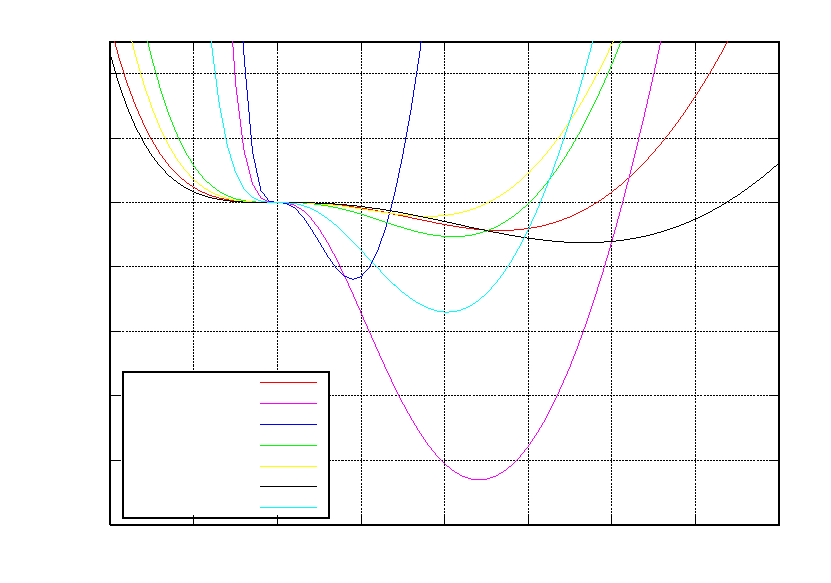
\includegraphics{grafico-ecuacion-4-zoom}}%
    \gplfronttext
  \end{picture}%
\endgroup

\end{figure}

Se puede observar que la función tiene dos raices, una en el 0 y la otra dependiendo de la muestra. 

Los $\beta$ hallados concuerdan con los resultados hallados aplicando los métodos.


%%%%%%%%%%%%%%%%%%%%%%%%%%%%%%%%%%%%%%%%%%%%%%%%%%%%%%%%%%%%%%%%%%%%%%%%%%%%%%%
%% Resultados                                                                %%
%%%%%%%%%%%%%%%%%%%%%%%%%%%%%%%%%%%%%%%%%%%%%%%%%%%%%%%%%%%%%%%%%%%%%%%%%%%%%%%


\section{Resultados}

A continuación presentamos el ajuste obtenido con la configuración que resultó ser más precisa:
Newton con mantisa de 51 bits de precisión, y cota de error absoluto 0.001.

\incluircsv{referencia.csv}
           {|c|c|c|c|}
           {Muestra & $\sigma$ & $\beta$ & $\lambda$}
           {\nombremuestra{\Muestra} & \Sigma & \Beta & \Lambda}

\subsection{Ajuste}

Algunos ejemplos del ajuste obtenido con los parámetros estimados.

\grafico{referencia-1.tex}{Muestra 1}
%\grafico{referencia-2.tex}{Muestra 2}
\grafico{referencia-3.tex}{Muestra 3}
%\grafico{referencia-4.tex}{Muestra 4}
%\grafico{referencia-5.tex}{Muestra 5}
%\grafico{referencia-6.tex}{Muestra 6}
%\grafico{referencia-7.tex}{Muestra 7}

\subsection{Gráficos comparativos}

El siguiente gráfico ilustra la curva de una distribución conocida, junto con las curvas de ajuste estimadas a partir de una muestra de la misma, usando ambos métodos de aproximación.

\begin{figure}[H]
  \centering
  \caption{Ajuste de una distribución conocida.}
  % GNUPLOT: LaTeX picture with Postscript
\begingroup
  \makeatletter
  \providecommand\color[2][]{%
    \GenericError{(gnuplot) \space\space\space\@spaces}{%
      Package color not loaded in conjunction with
      terminal option `colourtext'%
    }{See the gnuplot documentation for explanation.%
    }{Either use 'blacktext' in gnuplot or load the package
      color.sty in LaTeX.}%
    \renewcommand\color[2][]{}%
  }%
  \providecommand\includegraphics[2][]{%
    \GenericError{(gnuplot) \space\space\space\@spaces}{%
      Package graphicx or graphics not loaded%
    }{See the gnuplot documentation for explanation.%
    }{The gnuplot epslatex terminal needs graphicx.sty or graphics.sty.}%
    \renewcommand\includegraphics[2][]{}%
  }%
  \providecommand\rotatebox[2]{#2}%
  \@ifundefined{ifGPcolor}{%
    \newif\ifGPcolor
    \GPcolorfalse
  }{}%
  \@ifundefined{ifGPblacktext}{%
    \newif\ifGPblacktext
    \GPblacktexttrue
  }{}%
  % define a \g@addto@macro without @ in the name:
  \let\gplgaddtomacro\g@addto@macro
  % define empty templates for all commands taking text:
  \gdef\gplbacktext{}%
  \gdef\gplfronttext{}%
  \makeatother
  \ifGPblacktext
    % no textcolor at all
    \def\colorrgb#1{}%
    \def\colorgray#1{}%
  \else
    % gray or color?
    \ifGPcolor
      \def\colorrgb#1{\color[rgb]{#1}}%
      \def\colorgray#1{\color[gray]{#1}}%
      \expandafter\def\csname LTw\endcsname{\color{white}}%
      \expandafter\def\csname LTb\endcsname{\color{black}}%
      \expandafter\def\csname LTa\endcsname{\color{black}}%
      \expandafter\def\csname LT0\endcsname{\color[rgb]{1,0,0}}%
      \expandafter\def\csname LT1\endcsname{\color[rgb]{0,1,0}}%
      \expandafter\def\csname LT2\endcsname{\color[rgb]{0,0,1}}%
      \expandafter\def\csname LT3\endcsname{\color[rgb]{1,0,1}}%
      \expandafter\def\csname LT4\endcsname{\color[rgb]{0,1,1}}%
      \expandafter\def\csname LT5\endcsname{\color[rgb]{1,1,0}}%
      \expandafter\def\csname LT6\endcsname{\color[rgb]{0,0,0}}%
      \expandafter\def\csname LT7\endcsname{\color[rgb]{1,0.3,0}}%
      \expandafter\def\csname LT8\endcsname{\color[rgb]{0.5,0.5,0.5}}%
    \else
      % gray
      \def\colorrgb#1{\color{black}}%
      \def\colorgray#1{\color[gray]{#1}}%
      \expandafter\def\csname LTw\endcsname{\color{white}}%
      \expandafter\def\csname LTb\endcsname{\color{black}}%
      \expandafter\def\csname LTa\endcsname{\color{black}}%
      \expandafter\def\csname LT0\endcsname{\color{black}}%
      \expandafter\def\csname LT1\endcsname{\color{black}}%
      \expandafter\def\csname LT2\endcsname{\color{black}}%
      \expandafter\def\csname LT3\endcsname{\color{black}}%
      \expandafter\def\csname LT4\endcsname{\color{black}}%
      \expandafter\def\csname LT5\endcsname{\color{black}}%
      \expandafter\def\csname LT6\endcsname{\color{black}}%
      \expandafter\def\csname LT7\endcsname{\color{black}}%
      \expandafter\def\csname LT8\endcsname{\color{black}}%
    \fi
  \fi
  \setlength{\unitlength}{0.0500bp}%
  \begin{picture}(7678.00,5280.00)%
    \gplgaddtomacro\gplbacktext{%
      \colorrgb{0.00,0.00,0.00}%
      \put(860,640){\makebox(0,0)[r]{\strut{}0}}%
      \colorrgb{0.00,0.00,0.00}%
      \put(860,1190){\makebox(0,0)[r]{\strut{}0.01}}%
      \colorrgb{0.00,0.00,0.00}%
      \put(860,1740){\makebox(0,0)[r]{\strut{}0.02}}%
      \colorrgb{0.00,0.00,0.00}%
      \put(860,2290){\makebox(0,0)[r]{\strut{}0.03}}%
      \colorrgb{0.00,0.00,0.00}%
      \put(860,2840){\makebox(0,0)[r]{\strut{}0.04}}%
      \colorrgb{0.00,0.00,0.00}%
      \put(860,3389){\makebox(0,0)[r]{\strut{}0.05}}%
      \colorrgb{0.00,0.00,0.00}%
      \put(860,3939){\makebox(0,0)[r]{\strut{}0.06}}%
      \colorrgb{0.00,0.00,0.00}%
      \put(860,4489){\makebox(0,0)[r]{\strut{}0.07}}%
      \colorrgb{0.00,0.00,0.00}%
      \put(860,5039){\makebox(0,0)[r]{\strut{}0.08}}%
      \colorrgb{0.00,0.00,0.00}%
      \put(980,440){\makebox(0,0){\strut{}1.2}}%
      \colorrgb{0.00,0.00,0.00}%
      \put(1772,440){\makebox(0,0){\strut{}1.3}}%
      \colorrgb{0.00,0.00,0.00}%
      \put(2564,440){\makebox(0,0){\strut{}1.4}}%
      \colorrgb{0.00,0.00,0.00}%
      \put(3356,440){\makebox(0,0){\strut{}1.5}}%
      \colorrgb{0.00,0.00,0.00}%
      \put(4149,440){\makebox(0,0){\strut{}1.6}}%
      \colorrgb{0.00,0.00,0.00}%
      \put(4941,440){\makebox(0,0){\strut{}1.7}}%
      \colorrgb{0.00,0.00,0.00}%
      \put(5733,440){\makebox(0,0){\strut{}1.8}}%
      \colorrgb{0.00,0.00,0.00}%
      \put(6525,440){\makebox(0,0){\strut{}1.9}}%
      \colorrgb{0.00,0.00,0.00}%
      \put(7317,440){\makebox(0,0){\strut{}2}}%
      \colorrgb{0.00,0.00,0.00}%
      \put(160,2839){\rotatebox{90}{\makebox(0,0){\strut{}Frecuencia}}}%
      \colorrgb{0.00,0.00,0.00}%
      \put(4148,140){\makebox(0,0){\strut{}Muestra}}%
    }%
    \gplgaddtomacro\gplfronttext{%
      \csname LTb\endcsname%
      \put(6414,4876){\makebox(0,0)[r]{\strut{}Muestra}}%
      \csname LTb\endcsname%
      \put(6414,4676){\makebox(0,0)[r]{\strut{}Distribuci\'on conocida}}%
      \csname LTb\endcsname%
      \put(6414,4476){\makebox(0,0)[r]{\strut{}Newton}}%
      \csname LTb\endcsname%
      \put(6414,4276){\makebox(0,0)[r]{\strut{}Bisecci\'on}}%
    }%
    \gplbacktext
    \put(0,0){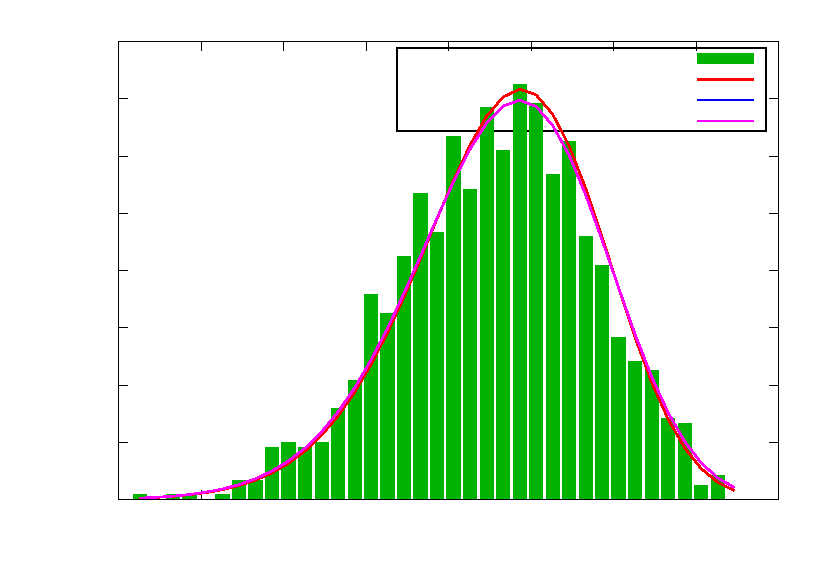
\includegraphics{grafico-distribucion-conocida}}%
    \gplfronttext
  \end{picture}%
\endgroup

\end{figure}

Las siguientes figuras ilustran distintos ajustes obtenidos haciendo variar algunos parámetros.

\subsubsection{Distintas precisiones de mantisa}

\grafico{biseccion-mantisas.tex}{Muestra 1: Método de Bisección}
\grafico{newton-mantisas.tex}{Muestra 1: Método de Newton}
             
\subsubsection{Distintos criterios de parada}

\grafico{biseccion-criterios-parada.tex}{Muestra 2: Método de Bisección}
\grafico{newton-criterios-parada.tex}{Muestra 2: Método de Newton}

\subsubsection{Promedio de iteraciones por método}

Promedios de las iteraciones realizadas con ambos métodos, diferentes cotas y criterios de parada.

\begin{figure}[H]
  \centering
  \caption{Iteraciones promedio}
  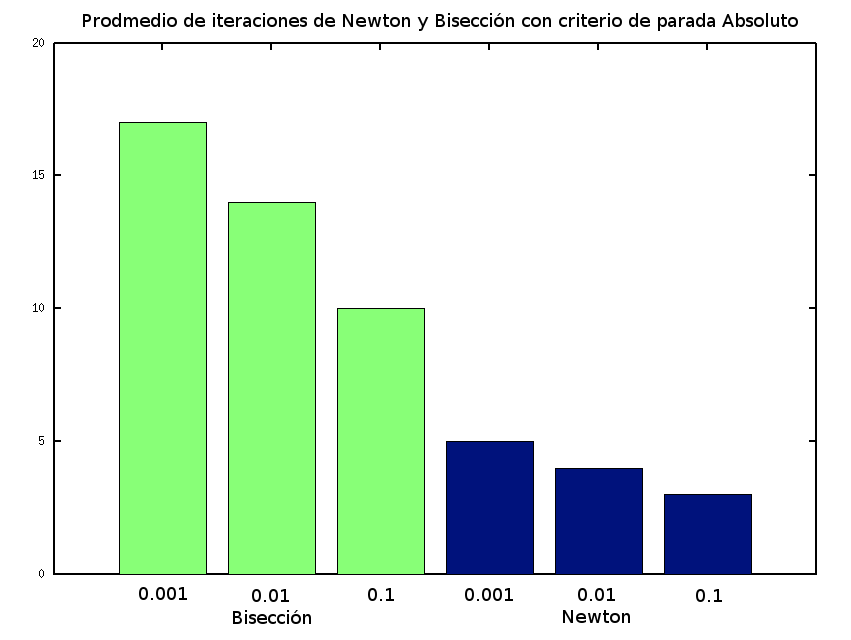
\includegraphics[width=140mm]{promItAbs.png}
\end{figure}

\begin{center}

\begin{tabular}{| c | c | c |  c | c | c |}
\hline
\multicolumn{3}{ |c| }{Bisección} & \multicolumn{3}{ |c| }{Newton} \\
\hline
17 & 0.001 & Absoluto & 5 & Absoluto & 0.001\\
14 & 0.01 & Absoluto & 4 & Absoluto & 0.01\\
10 & 0.1 & Absoluto  & 3 & Absoluto & 0.1\\
15 & 0.001 & Relativo & 5 & Relativo & 0.001\\
12 & 0.01 & Relativo & 3 & Relativo & 0.01\\
9 & 0.1 & Relativo & 2 & Relativo & 0.1\\
\hline
\end{tabular}

\end{center}
%%%%%%%%%%%%%%%%%%%%%%%%%%%%%%%%%%%%%%%%%%%%%%%%%%%%%%%%%%%%%%%%%%%%%%%%%%%%%%%
%% Discusión                                                                 %%
%%%%%%%%%%%%%%%%%%%%%%%%%%%%%%%%%%%%%%%%%%%%%%%%%%%%%%%%%%%%%%%%%%%%%%%%%%%%%%%


\section{Discusión}

Analizamos a continuación las diferencias observadas al variar métodos, cotas
de error, criterios de parada y bits de precisión de mantisa.


\subsection{Métodos de aproximación}
Para precisión de mantisa alta y cota de error chica, se observa una muy pequeña
mejora en el ajuste al aproximar con Newton, practicamente indistinguible a simple
vista. Sin embargo la brecha en el ajuste se hace más notable al decrementar
los parámetros mencionados. Ver figuras 8, 9, 10 y 11.

En la mayoría de los casos el método de bisección requiere una mayor cantidad
de iteraciones, a veces más del doble que la requeida por Newton.


\subsection{Criterios de parada y cotas de error}
Observamos una mejora numérica notable comparando las cotas de error absoluto 0.1 y 0.01,
pero prácticamente despreciable comparando con 0.001. Sin embargo, el ajuste
obtenido con cota 0.1 es excelente, y decrementar la cota produce cambios en
el ajuste casi indistinguibles a simple vista. Lo mismo ocurre con cotas de error relativo.

La figura 9 ilustra la diferencia de ajuste con cotas de error relativo 0.1 vs 0.001,
donde la diferencia entre las curvas es pequeñísima, sin embargo los parámetros
$\beta$ obtenidos difieren mucho entre sí: 4.48047 vs 4.12698, respectivamente.

Observando la Figura 10, podemos observar las diferencias entre las cantidades de iteraciones. En ambos método, el criterio de parada \textit{Relativo} obtuvo la menor cantidad de iteraciones. También se comprueba que el aumento de precisión (\textit{Cota de error}) implica un aumento de iteraciones. Al ser la convergencia del método de \textit{Bisección} lineal, el aumento de las iteraciones es mayor que en \textit{Newton}.

\subsection{Bits de precisión en mantisa}
No observamos mejoras significativas de ajuste al incrementar la precisión de
la mantisa por encima de 20 bits. Sin embargo, observamos gran deterioro en el
ajuste al emplear mantisas de menos de 15 bits, claramente visible en las figuras
8 y 9.


%%%%%%%%%%%%%%%%%%%%%%%%%%%%%%%%%%%%%%%%%%%%%%%%%%%%%%%%%%%%%%%%%%%%%%%%%%%%%%%
%% Conclusiones                                                              %%
%%%%%%%%%%%%%%%%%%%%%%%%%%%%%%%%%%%%%%%%%%%%%%%%%%%%%%%%%%%%%%%%%%%%%%%%%%%%%%%


\section{Conclusiones}

Determinamos que tanto el método de bisección como Newton son suficientes para
alcanzar aproximaciones adecuadas.

Observamos que la configuración que minimiza el número de iteraciones y la
cantidad requerida de bits de precisiónde mantisa para el corpus analizado es
aplicar Newton con 20 bits de precisión y cota de error absoluto 0.1.

No observamos mejoras significativas al aumentar la precisión de mantisa o
decrementar la cota de error.

Encontramos un enfoque híbrido aplicando inicialmente bisección con una cota de
error grosera para hallar una aproximación inicial, para luego aplicar Newton y
mejorar las chances de converger a una solución.

Finalmente, nos queda pendiente explorar otros  métodos de aproximación existentes
(ej: método de la secante y regula falsi.)


%%%%%%%%%%%%%%%%%%%%%%%%%%%%%%%%%%%%%%%%%%%%%%%%%%%%%%%%%%%%%%%%%%%%%%%%%%%%%%%
%% Apéndice A: Enunciado del Trabajo Práctico                                %%
%%%%%%%%%%%%%%%%%%%%%%%%%%%%%%%%%%%%%%%%%%%%%%%%%%%%%%%%%%%%%%%%%%%%%%%%%%%%%%%


\section{Apéndice A: Enunciado del Trabajo Práctico}

\newcommand{\real}{\mathbb{R}}
\newcommand{\nat}{\mathbb{N}}
\newcommand{\eme}{\mathcal{M}}
\newcommand{\emeh}{\widehat{\mathcal{M}}}
\newcommand{\ere}{\mathcal{R}}

\subsection{Introducci\'on}

Numerosas aplicaciones utilizan la distribuci\'on Gamma Generalizada (D$\Gamma$G) para modelar datos, cuya funci\'on de densidad se expresa como $$f_\Theta(x)=\frac{\beta\, x^{\beta \lambda - 1}}{\sigma^{\beta \lambda}\, \Gamma(\lambda)} \exp\left\{-\left(\frac{x}{\sigma} \right)^\beta \right\}\qquad\textrm{con } x\in\real_{>0}$$ donde 
$\Gamma(\cdot)$ es la funci\'on Gamma\footnote{La funci\'on Gamma, en el caso entero, es equivalente a la funci\'on factorial: $\Gamma(n)=n!$, $\forall n\in\nat$ } definida como $\Gamma(z)=\int_0^{\infty}{t^{z-1}e^{-t}\,dt}$, y $\Theta$ representa a la tupla de par\'ametros $\Theta=(\sigma,\beta,\lambda)$. El primero se encuentra relacionado con la escala de la funci\'on $f$ y los otros dos con la forma; todos son positivos.
La D$\Gamma$G engloba un conjunto amplio de distribuciones param\'etricas, donde la distribuci\'on exponencial, Weibull o Gamma son casos especiales de \'esta.
En vez de utilizar (y almacenar) el histograma emp\'irico de los datos, representarlos solamente con los par\'ametros de esta distribuci\'on resulta ser, en muchos casos, una opci\'on m\'as que conveniente. El problema que surge consiste en estimar de forma certera y eficiente los par\'ametros de la D$\Gamma$G que mejor ajusta a los datos.

\subsection{Estimaci\'on de par\'ametros}

Sean $n$ datos reales positivos $x_1,\dots,x_n$. Estos datos pueden provenir de mediciones de un sat\'elite, p\'ixeles de im\'agenes, etc., y de los cuales asumimos que siguen una distribuci\'on D$\Gamma$G cuyos par\'ametros queremos estimar. Como se vi\'o en la materia \emph{Proba}, existen m\'etodos como `\textsl{estimadores de m\'axima verosimilitud'}, donde a partir de las muestras se pueden estimar par\'ametros de distribuciones. Utilizando este m\'etodo, llegamos a que se deben cumplir las siguientes condiciones:
\begin{eqnarray}
\tilde{\sigma} & = & \left(\frac{\sum_{i=1}^n{x_i^{\tilde{\beta}}}}{n \tilde{\lambda}} \right)^{1/\tilde{\beta}} \label{eqn:sigma}\\
\tilde{\lambda} & = &\left[ \tilde{\beta} \left( \frac{\sum_{i=1}^n{x_i^{\tilde{\beta}} \log x_i}}{\sum_{i=1}^n{x_i^{\tilde{\beta}}}} - \frac{\sum_{i=1}^n{\log x_i}}{n} \right)\right]^{-1} \label{eqn:lambda}\\
 0 & = & \frac{\tilde{\beta}}{n} \sum_{i=1}^n{\log x_i} - \log {\sum_{i=1}^n{x_i^{\tilde{\beta}}}} + \log(n \tilde{\lambda}) - \psi(\tilde{\lambda})
\end{eqnarray}
donde $\tilde{\Theta}=(\tilde{\sigma},\tilde{\beta},\tilde{\lambda})$ son las estimaciones a partir de las muestras de datos y $\psi(\cdot)$ es la `conocida' funci\'on digamma\footnote{$\psi(z) = \frac{\partial}{\partial z} \ln \Gamma (z) = \frac{\Gamma'(z)}{\Gamma(z)}$.} que se define como la derivada logar\'itmica de la funci\'on Gamma. Notar que una una vez estimado el par\'ametro $\beta$, los otros dos par\'ametros pueden obtenerse de las primeras dos ecuaciones. A partir del c\'alculo de los \textsl{momentos} de una variable aleatoria con funci\'on de densidad $f_\Theta(x)$ se pueden obtener las siguientes dos ecuaciones:
\begin{eqnarray}
\log(\eme(2\beta)) -2\log(\eme(\beta)) & = & \log(1+\beta(\ere(\beta)-\ere(0))) \label{eqn:sol1}\\
\frac{\eme(2\beta)}{\eme^2(\beta)} & = & 1+\beta(\ere(\beta)-\ere(0))) \label{eqn:sol2}
\end{eqnarray}
donde 
$$\eme(s) =  \frac{1}{n}\sum_{i=1}^n{x_i^s}\,, \qquad \emeh(s) = \frac{1}{n}\sum_{i=1}^n{x_i^s \log(x_i)}\,,  \qquad \ere(s) = \frac{\emeh(s)}{\eme(s)}$$
Estas ecuaciones tienen como ventaja que no dependen de los otros par\'ametros, utiliz\'andose funciones m\'as sencillas que s\'olo dependen de los datos. Hallando la soluci\'on de cualquiera de las ecuaciones (\ref{eqn:sol1}) o (\ref{eqn:sol2}), es posible estimar el par\'ametro $\beta$, y despejar el resto de los par\'ametros utilizando las ecuaciones (\ref{eqn:sigma}) y (\ref{eqn:lambda}).

\subsection{Enunciado}

El objetivo del trabajo pr\'actico es implementar un programa que permita estimar los par\'ametros $\Theta=(\sigma,\beta,\lambda)$ a partir de un conjunto de $n$ datos. Para ello, se deber\'a resolver la ecuaciones (\ref{eqn:sol1}) o (\ref{eqn:sol2}).
Evaluando los distintos m\'etodos vistos en clase que permitan resolver este problema, se deber\'a realizar una implementaci\'on cumpliendo lo siguiente:

\begin{enumerate} 
\item Implementar al menos dos m\'etodos (de los cuales uno de ellos debe ser el m\'etodo de Newton) con aritm\'etica binaria de punto flotante con $t$ d\'igitos de precisi\'on en la mantisa. El valor $t$ debe ser un par\'ametro de la implementaci\'on, con $t<52$.
\item  Realizar experimentos num\'ericos con cada m\'etodo implementado en el \'item anterior elegiendo varias instancias de prueba y en funci\'on de las cantidad de d\'igitos $t$ de precisi\'on en la mantisa (experimentar con al menos 3 valores distintos de $t$).
\item Para cada m\'etodo implementado se deber\'an mostrar resultados obtenidos en cuanto a cantidad necesaria de iteraciones, tiempo de ejecuci\'on, precisi\'on en el resultado, y cualquier otro par\'ametro que considere de inter\'es evaluar.
\item Realizar el gr\'afico del histograma de los datos y el ajuste obtenido. Extraer conclusiones sobre la efectividad de cada m\'etodo observando los resultados anteriores.  
\end{enumerate}

\subsection{Formato de archivos de entrada}

El programa debe tomar los datos desde un archivo de texto con el siguiente formato:

\vspace{0.5cm}

\begin{tabular}{|l|} \hline 
\verb|input_file.txt|\\ \hline
\verb|n|\\ 
$\mathtt{x_1\ x_2\ \ldots\ x_n}$ \\ \hline
\end{tabular}

\vspace{0.5cm}

El archivo contiene en la primer l\'inea la cantidad de datos, y en la l\'inea siguiente se encuentran los $n$ datos (reales positivos) separados por espacio. En la web de la materia se publicar\'an varios archivos de prueba para realizar los primeros experimentos.

\subsection{Fecha de entrega:} 

\begin{itemize}
\item \textsl{Formato electr\'onico:} domingo 14 de abril de 2013, hasta las 23:59 hs., enviando el trabajo (informe+c\'odigo) a \texttt{metnum.lab@gmail.com}. El subject del email debe comenzar con el texto \verb|[TP1]| seguido de la lista de apellidos de los integrantes del grupo. 
\item \textsl{Formato f\'isico:} lunes 15 de abril de 2013, de 18 a 20hs (en la clase pr\'actica).
\end{itemize}


%%%%%%%%%%%%%%%%%%%%%%%%%%%%%%%%%%%%%%%%%%%%%%%%%%%%%%%%%%%%%%%%%%%%%%%%%%%%%%%
%% Apéndice B: Tablas de Aproximaciones                                      %%
%%%%%%%%%%%%%%%%%%%%%%%%%%%%%%%%%%%%%%%%%%%%%%%%%%%%%%%%%%%%%%%%%%%%%%%%%%%%%%%


\section{Apéndice B: Tablas de Aproximaciones}

\newcommand{\csvmuestra}[1]{
    \incluircsv{#1}
               {|c|c|c|c|c|c|c|}
               {$\sigma$ & $\beta$ & $\lambda$ & Iteraciones & Criterio de parada & Cota & Mantisa}
               {\Sigma & \Beta & \Lambda & \Iteraciones & Error \CritParada & \CotaError & \BitsMantisa{ }bits}    
}

\subsection{Método de bisección}
Resultados con distintas precisiones y cotas de error usando  método de bisección.

\subsubsection{Muestra 1}
\csvmuestra{ biseccion-1.csv}

%\subsubsection{Muestra 2}
%\csvmuestra{ biseccion-2.csv}

\subsubsection{Muestra 3}
\csvmuestra{ biseccion-3.csv}

%\subsubsection{Muestra 4}
%\csvmuestra{ biseccion-4.csv}

%\subsubsection{Muestra 5}
%\csvmuestra{ biseccion-5.csv}

%\subsubsection{Muestra 6}
%\csvmuestra{ biseccion-6.csv}

%\subsubsection{Muestra 7}
%\csvmuestra{ biseccion-7.csv}


\subsection{Método de Newton}
Resultados con distintas precisiones y cotas de error usando  método de Newton.

\subsubsection{Muestra 1}
\csvmuestra{    newton-1.csv}

%\subsubsection{Muestra 2}
%\csvmuestra{    newton-2.csv}

\subsubsection{Muestra 3}
\csvmuestra{    newton-3.csv}

%\subsubsection{Muestra 4}
%\csvmuestra{    newton-4.csv}

%\subsubsection{Muestra 5}
%\csvmuestra{    newton-5.csv}

%\subsubsection{Muestra 6}
%\csvmuestra{    newton-6.csv}

%\subsubsection{Muestra 7}
%\csvmuestra{    newton-7.csv}


%%%%%%%%%%%%%%%%%%%%%%%%%%%%%%%%%%%%%%%%%%%%%%%%%%%%%%%%%%%%%%%%%%%%%%%%%%%%%%%
%% Apéndice C: Código Fuente                                                 %%
%%%%%%%%%%%%%%%%%%%%%%%%%%%%%%%%%%%%%%%%%%%%%%%%%%%%%%%%%%%%%%%%%%%%%%%%%%%%%%%


\section{Apéndice C: Código Fuente}


\subsection{Requerimientos}

Compilador g++ y GNU Make.


\subsection{Instrucciones}

Compilar el programa ejecutando \texttt{make} en el directorio raíz del proyecto.

Luego de compilar, tipear \texttt{./dgg} en el directorio raíz para invocar el
binario y obtener ayuda en pantalla.


\subsection{Metodos.h}
\lstinputlisting[language=C++]{../src/Metodos.h}


\subsection{Metodos.cpp}
\lstinputlisting[language=C++]{../src/Metodos.cpp}


\subsection{Ecuaciones.cpp}
\lstinputlisting[language=C++]{../src/Ecuaciones.cpp}


%%%%%%%%%%%%%%%%%%%%%%%%%%%%%%%%%%%%%%%%%%%%%%%%%%%%%%%%%%%%%%%%%%%%%%%%%%%%%%%
%% Bibliografía                                                              %%
%%%%%%%%%%%%%%%%%%%%%%%%%%%%%%%%%%%%%%%%%%%%%%%%%%%%%%%%%%%%%%%%%%%%%%%%%%%%%%%


\begin{thebibliography}{1}
    \bibitem[Burden2010]{burden}
        Richard L. Burden,
        J. Douglas Faires,
        \emph{Numerical Analysis}.
        Brooks/Cole,
        Ninth Edition,
        2010.
\end{thebibliography}

\end{document}